\documentclass{article}
\usepackage{listings}
\usepackage[paperwidth=10in, paperheight=10in]{geometry}

\lstset{basicstyle=\ttfamily}
\usepackage{tikz}
\usetikzlibrary{automata,positioning}
\begin{document}

\begin{itemize}
\item DELIM: \verb$/[{}\(\);\[\]]/$

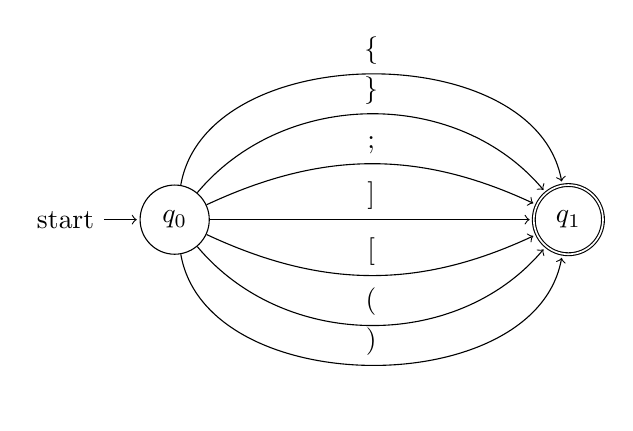
\begin{tikzpicture}[shorten >=1pt,node distance=5cm,on grid,auto] 
   \node[state,initial] (q0)   {$q_0$}; 
   \node[state,accepting](q1) [right=of q0] {$q_1$};
    \path[->] 
    (q0) edge[bend left=80]   node {\{} (q1)
    (q0) edge[bend left=50]   node {\}} (q1)
    (q0) edge[bend right=50]  node {(} (q1)
    (q0) edge[bend right=80]  node {)} (q1)
    (q0) edge[bend left=25]   node {;} (q1)
    (q0) edge[bend right=25]  node {[} (q1)
    (q0) edge                 node {]} (q1);
\end{tikzpicture}


\item SPACE: \verb$/[ \t\r\n\v\f]+/$

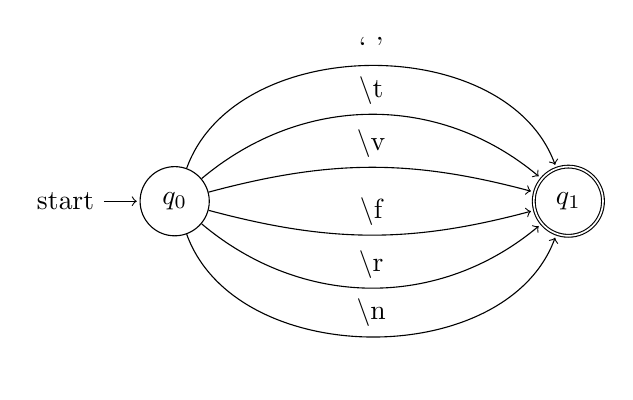
\begin{tikzpicture}[shorten >=1pt,node distance=5cm,on grid,auto] 
   \node[state,initial] (q0)   {$q_0$}; 
   \node[state,accepting](q1) [right=of q0] {$q_1$};
    \path[->] 
    (q0) edge[bend left=70]   node {` '} (q1)
    (q0) edge[bend left=40]   node {$\backslash$t} (q1)
    (q0) edge[bend right=40]  node {$\backslash$r} (q1)
    (q0) edge[bend right=70]  node {$\backslash$n} (q1)
    (q0) edge[bend left=15]   node {$\backslash$v} (q1)
    (q0) edge[bend right=15]  node {$\backslash$f} (q1);
\end{tikzpicture}

\item IDENT: \verb$/[a-zA-Z_][a-zA-Z0-9_]*/$

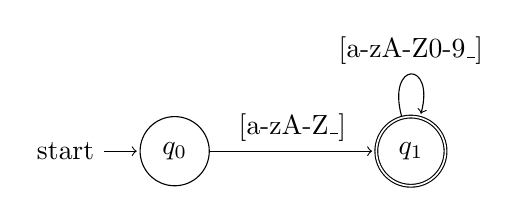
\begin{tikzpicture}[shorten >=1pt,node distance=3cm,on grid,auto] 
   \node[state,initial] (q0)   {$q_0$}; 
   \node[state,accepting](q1) [right=of q0] {$q_1$};
    \path[->] 
    (q0) edge  node {[a-zA-Z\_]} (q1)
    (q1) edge [loop above] node {[a-zA-Z0-9\_]} (q1);
\end{tikzpicture}

\item INTEGER: \verb$/[0-9]+/$

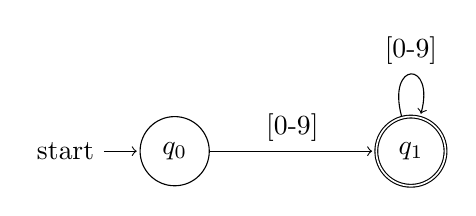
\begin{tikzpicture}[shorten >=1pt,node distance=3cm,on grid,auto] 
   \node[state,initial] (q0)   {$q_0$}; 
   \node[state,accepting](q1) [right=of q0] {$q_1$};
    \path[->] 
    (q0) edge  node {[0-9]} (q1)
    (q1) edge [loop above] node {[0-9]} (q1);
\end{tikzpicture}


\item FLOAT: \verb$/[0-9]*\.[0-9]+/$

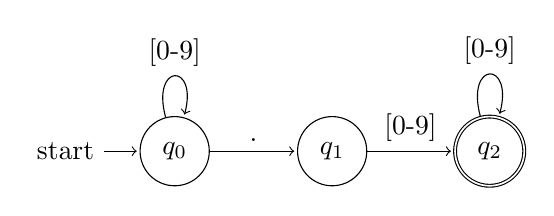
\begin{tikzpicture}[shorten >=1pt,node distance=2cm,on grid,auto] 
   \node[state,initial] (q0)   {$q_0$}; 
   \node[state](q1) [right=of q0] {$q_1$};
   \node[state,accepting](q2) [right=of q1] {$q_2$};
    \path[->] 
    (q0) edge  node {.} (q1)
    (q1) edge  node {[0-9]} (q2)
    (q0) edge [loop above] node {[0-9]} (q0)
    (q2) edge [loop above] node {[0-9]} (q2);
\end{tikzpicture}

\item CHAR: \verb$/\'(?:[\x20-\x5B\x5D-\x7E]|\\[abtnvfre\\])\'/$ 

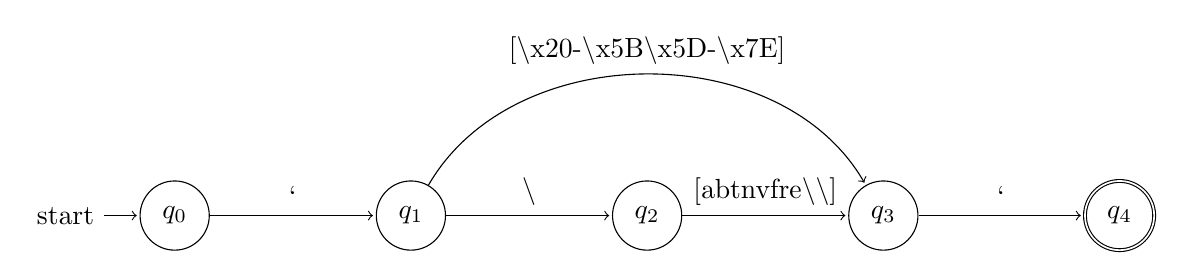
\begin{tikzpicture}[shorten >=1pt,node distance=3cm,on grid,auto] 
   \node[state,initial] (q0)   {$q_0$}; 
   \node[state] (q1) [right=of q0] {$q_1$}; 
   \node[state] (q2) [right=of q1] {$q_2$}; 
   \node[state] (q3) [right=of q2] {$q_3$}; 
   \node[state, accepting] (q4) [right=of q3] {$q_4$}; 
    \path[->] 
    (q0) edge  node {$`$} (q1)
    (q1) edge[bend left=60] node {
        [$\backslash$x20-$\backslash$x5B$\backslash$x5D-$\backslash$x7E]
    } (q3)
    (q1) edge node {$\backslash$} (q2)
    (q2) edge node {[abtnvfre$\backslash\backslash$]} (q3)
    (q3) edge  node {$`$} (q4);
\end{tikzpicture}

\item STRING: \verb$/\"(?:[^"]|\\\")*\"/$

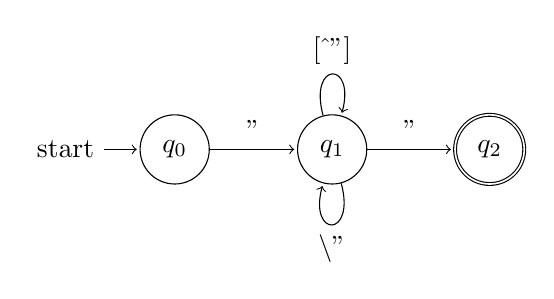
\begin{tikzpicture}[shorten >=1pt,node distance=2cm,on grid,auto] 
   \node[state,initial] (q0)   {$q_0$}; 
   \node[state] (q1) [right=of q0] {$q_1$}; 
   \node[state, accepting] (q2) [right=of q1] {$q_2$}; 
    \path[->] 
    (q0) edge  node {$"$} (q1)
    (q1) edge [loop above] node {$[\hat{~}"]$} (q1)
         edge [loop below] node {$\backslash"$} (q1)

    (q1) edge  node {$"$} (q2);
\end{tikzpicture}


\item OPER: \verb$/(?:[\+\-\*\/%=!<>]=?)/$

\begin{tikzpicture}[shorten >=1pt,node distance=7cm,on grid,auto] 
    \node[state,initial] (q0)   {$q_0$}; 
    \node[state,accepting](q1) [right=of q0] {$q_1$};
    \node[state,accepting](q2) [right=of q2] {$q_2$};
    \path[->] 
    (q0) edge   node {$+$} (q1)
    (q0) edge[bend right=65]  node {$-$} (q1)
    (q0) edge[bend left=65]   node {$*$} (q1)
    (q0) edge[bend right=45]  node {$/$} (q1)
    (q0) edge[bend left=45]   node {$\%$} (q1)
    (q0) edge[bend right=30]  node {$!$} (q1)
    (q0) edge[bend left=30]   node {$<$} (q1)
    (q0) edge[bend left=15]   node {$>$} (q1)
    (q0) edge[bend right=15]  node {$=$} (q1)
    (q1) edge   node {$=$} (q2);
\end{tikzpicture}

\item ALL: 
    
    \begin{itemize}
        \item C\_DELIM $= [91, 93, 123, 125, 40, 41, 59]$
        \item C\_SPACE $= [32, 9, 10, 11, 12, 13]$
        \item C\_OPER  $= [42, 37, 60, 62, 43, 61, 33, 47, 45]$
        \item C\_LETTERS  $= [65, \dots, 90, 97, \dots, 122, 95]$
        \item C\_NUMBERS  $= [48, 57]$
        
    \end{itemize}
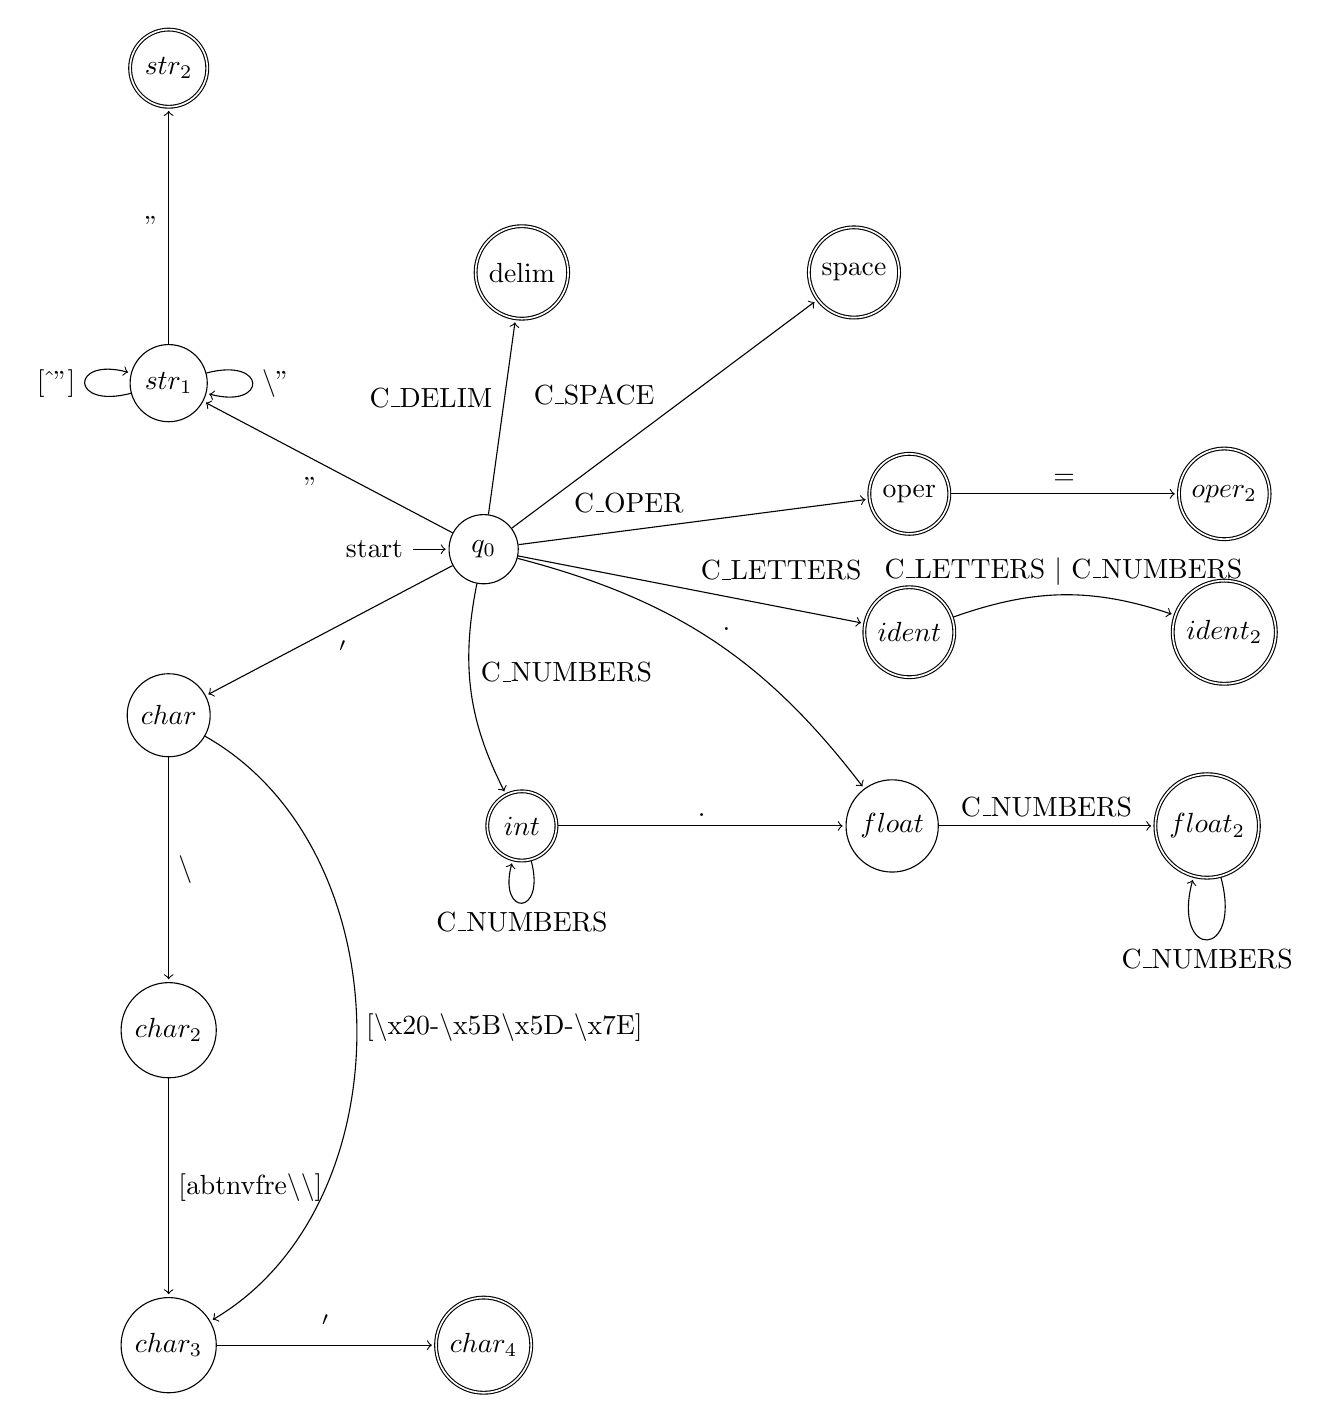
\begin{tikzpicture}[shorten >=1pt,node distance=4cm,on grid,auto] 
    \node[state,initial] (q0)   {$q_0$}; 
    \node[state,accepting](delim) [right=of q0, yshift=100, xshift=-100] {delim};
    \node[state,accepting](space) [right=of q0, yshift=100, xshift=20] {space};
    \node[state,accepting](oper) [right=of q0, yshift=20, xshift=40] {oper};
    \node[state,accepting](oper2) [right=of oper] {$oper_2$};
    \node[state,accepting](ident) [right=of q0, yshift=-30, xshift=40] {$ident$};
    \node[state,accepting](ident2) [right=of ident] {$ident_2$};
    \node[state,accepting](integ) [right=of q0, yshift=-100, xshift=-100] {$int$};
    \node[state](float) [right=of integ, xshift=20] {$float$};
    \node[state,accepting](float2) [right=of float] {$float_2$};
    \node[state] (char1) [left=of q0, yshift=-60] {$char$}; 
    \node[state] (char2) [below=of char1] {$char_2$}; 
    \node[state] (char3) [below=of char2] {$char_3$}; 
    \node[state, accepting] (char4) [right=of char3] {$char_4$}; 
    \node[state] (str1) [left=of q0, yshift=60] {$str_1$}; 
    \node[state, accepting] (str2) [above=of str1] {$str_2$};
    \path[->] 

    (q0) edge node {C\_DELIM} (delim)
    (q0) edge node {C\_SPACE} (space)
    (q0) edge node {C\_OPER} (oper)
    (oper) edge node {$=$} (oper2)
    (q0) edge node {C\_LETTERS} (ident)
    (ident) edge [bend left=19] node {C\_LETTERS $|$ C\_NUMBERS} (ident2)
    (q0) edge [bend right=19] node {C\_NUMBERS} (integ)
    (integ) edge [loop below] node {C\_NUMBERS} (integ)
    (q0) edge  [bend left=19] node {$.$} (float)
    (integ) edge node {$.$} (float)
    (float) edge  node {C\_NUMBERS} (float2)
    (float2) edge [loop below] node {C\_NUMBERS} (float2)
    (q0) edge  node {$'$} (char1)
    (char1) edge[bend left=60] node { %
        [$\backslash$x20-$\backslash$x5B$\backslash$x5D-$\backslash$x7E] %
    } (char3) 
    (char1) edge node {$\backslash$} (char2)
    (char2) edge node {[abtnvfre$\backslash\backslash$]} (char3)
    (char3) edge  node {$'$} (char4)
    (q0) edge  node {$"$} (str1)
    (str1) edge [loop left] node {$[\hat{~}"]$} (str1)
           edge [loop right] node {$\backslash"$} (str1)
           edge  node {$"$} (str2);
\end{tikzpicture}







\end{itemize}
\end{document}  
